\documentclass[1p]{elsarticle_modified}
%\bibliographystyle{elsarticle-num}

%\usepackage[colorlinks]{hyperref}
%\usepackage{abbrmath_seonhwa} %\Abb, \Ascr, \Acal ,\Abf, \Afrak
\usepackage{amsfonts}
\usepackage{amssymb}
\usepackage{amsmath}
\usepackage{amsthm}
\usepackage{scalefnt}
\usepackage{amsbsy}
\usepackage{kotex}
\usepackage{caption}
\usepackage{subfig}
\usepackage{color}
\usepackage{graphicx}
\usepackage{xcolor} %% white, black, red, green, blue, cyan, magenta, yellow
\usepackage{float}
\usepackage{setspace}
\usepackage{hyperref}

\usepackage{tikz}
\usetikzlibrary{arrows}

\usepackage{multirow}
\usepackage{array} % fixed length table
\usepackage{hhline}

%%%%%%%%%%%%%%%%%%%%%
\makeatletter
\renewcommand*\env@matrix[1][\arraystretch]{%
	\edef\arraystretch{#1}%
	\hskip -\arraycolsep
	\let\@ifnextchar\new@ifnextchar
	\array{*\c@MaxMatrixCols c}}
\makeatother %https://tex.stackexchange.com/questions/14071/how-can-i-increase-the-line-spacing-in-a-matrix
%%%%%%%%%%%%%%%

\usepackage[normalem]{ulem}

\newcommand{\msout}[1]{\ifmmode\text{\sout{\ensuremath{#1}}}\else\sout{#1}\fi}
%SOURCE: \msout is \stkout macro in https://tex.stackexchange.com/questions/20609/strikeout-in-math-mode

\newcommand{\cancel}[1]{
	\ifmmode
	{\color{red}\msout{#1}}
	\else
	{\color{red}\sout{#1}}
	\fi
}

\newcommand{\add}[1]{
	{\color{blue}\uwave{#1}}
}

\newcommand{\replace}[2]{
	\ifmmode
	{\color{red}\msout{#1}}{\color{blue}\uwave{#2}}
	\else
	{\color{red}\sout{#1}}{\color{blue}\uwave{#2}}
	\fi
}

\newcommand{\Sol}{\mathcal{S}} %segment
\newcommand{\D}{D} %diagram
\newcommand{\A}{\mathcal{A}} %arc


%%%%%%%%%%%%%%%%%%%%%%%%%%%%%5 test

\def\sl{\operatorname{\textup{SL}}(2,\Cbb)}
\def\psl{\operatorname{\textup{PSL}}(2,\Cbb)}
\def\quan{\mkern 1mu \triangleright \mkern 1mu}

\theoremstyle{definition}
\newtheorem{thm}{Theorem}[section]
\newtheorem{prop}[thm]{Proposition}
\newtheorem{lem}[thm]{Lemma}
\newtheorem{ques}[thm]{Question}
\newtheorem{cor}[thm]{Corollary}
\newtheorem{defn}[thm]{Definition}
\newtheorem{exam}[thm]{Example}
\newtheorem{rmk}[thm]{Remark}
\newtheorem{alg}[thm]{Algorithm}

\newcommand{\I}{\sqrt{-1}}
\begin{document}

%\begin{frontmatter}
%
%\title{Boundary parabolic representations of knots up to 8 crossings}
%
%%% Group authors per affiliation:
%\author{Yunhi Cho} 
%\address{Department of Mathematics, University of Seoul, Seoul, Korea}
%\ead{yhcho@uos.ac.kr}
%
%
%\author{Seonhwa Kim} %\fnref{s_kim}}
%\address{Center for Geometry and Physics, Institute for Basic Science, Pohang, 37673, Korea}
%\ead{ryeona17@ibs.re.kr}
%
%\author{Hyuk Kim}
%\address{Department of Mathematical Sciences, Seoul National University, Seoul 08826, Korea}
%\ead{hyukkim@snu.ac.kr}
%
%\author{Seokbeom Yoon}
%\address{Department of Mathematical Sciences, Seoul National University, Seoul, 08826,  Korea}
%\ead{sbyoon15@snu.ac.kr}
%
%\begin{abstract}
%We find all boundary parabolic representation of knots up to 8 crossings.
%
%\end{abstract}
%\begin{keyword}
%    \MSC[2010] 57M25 
%\end{keyword}
%
%\end{frontmatter}

%\linenumbers
%\tableofcontents
%
\newcommand\colored[1]{\textcolor{white}{\rule[-0.35ex]{0.8em}{1.4ex}}\kern-0.8em\color{red} #1}%
%\newcommand\colored[1]{\textcolor{white}{ #1}\kern-2.17ex	\textcolor{white}{ #1}\kern-1.81ex	\textcolor{white}{ #1}\kern-2.15ex\color{red}#1	}

{\Large $\underline{12a_{0087}~(K12a_{0087})}$}

\setlength{\tabcolsep}{10pt}
\renewcommand{\arraystretch}{1.6}
\vspace{1cm}\begin{tabular}{m{100pt}>{\centering\arraybackslash}m{274pt}}
\multirow{5}{120pt}{
	\centering
	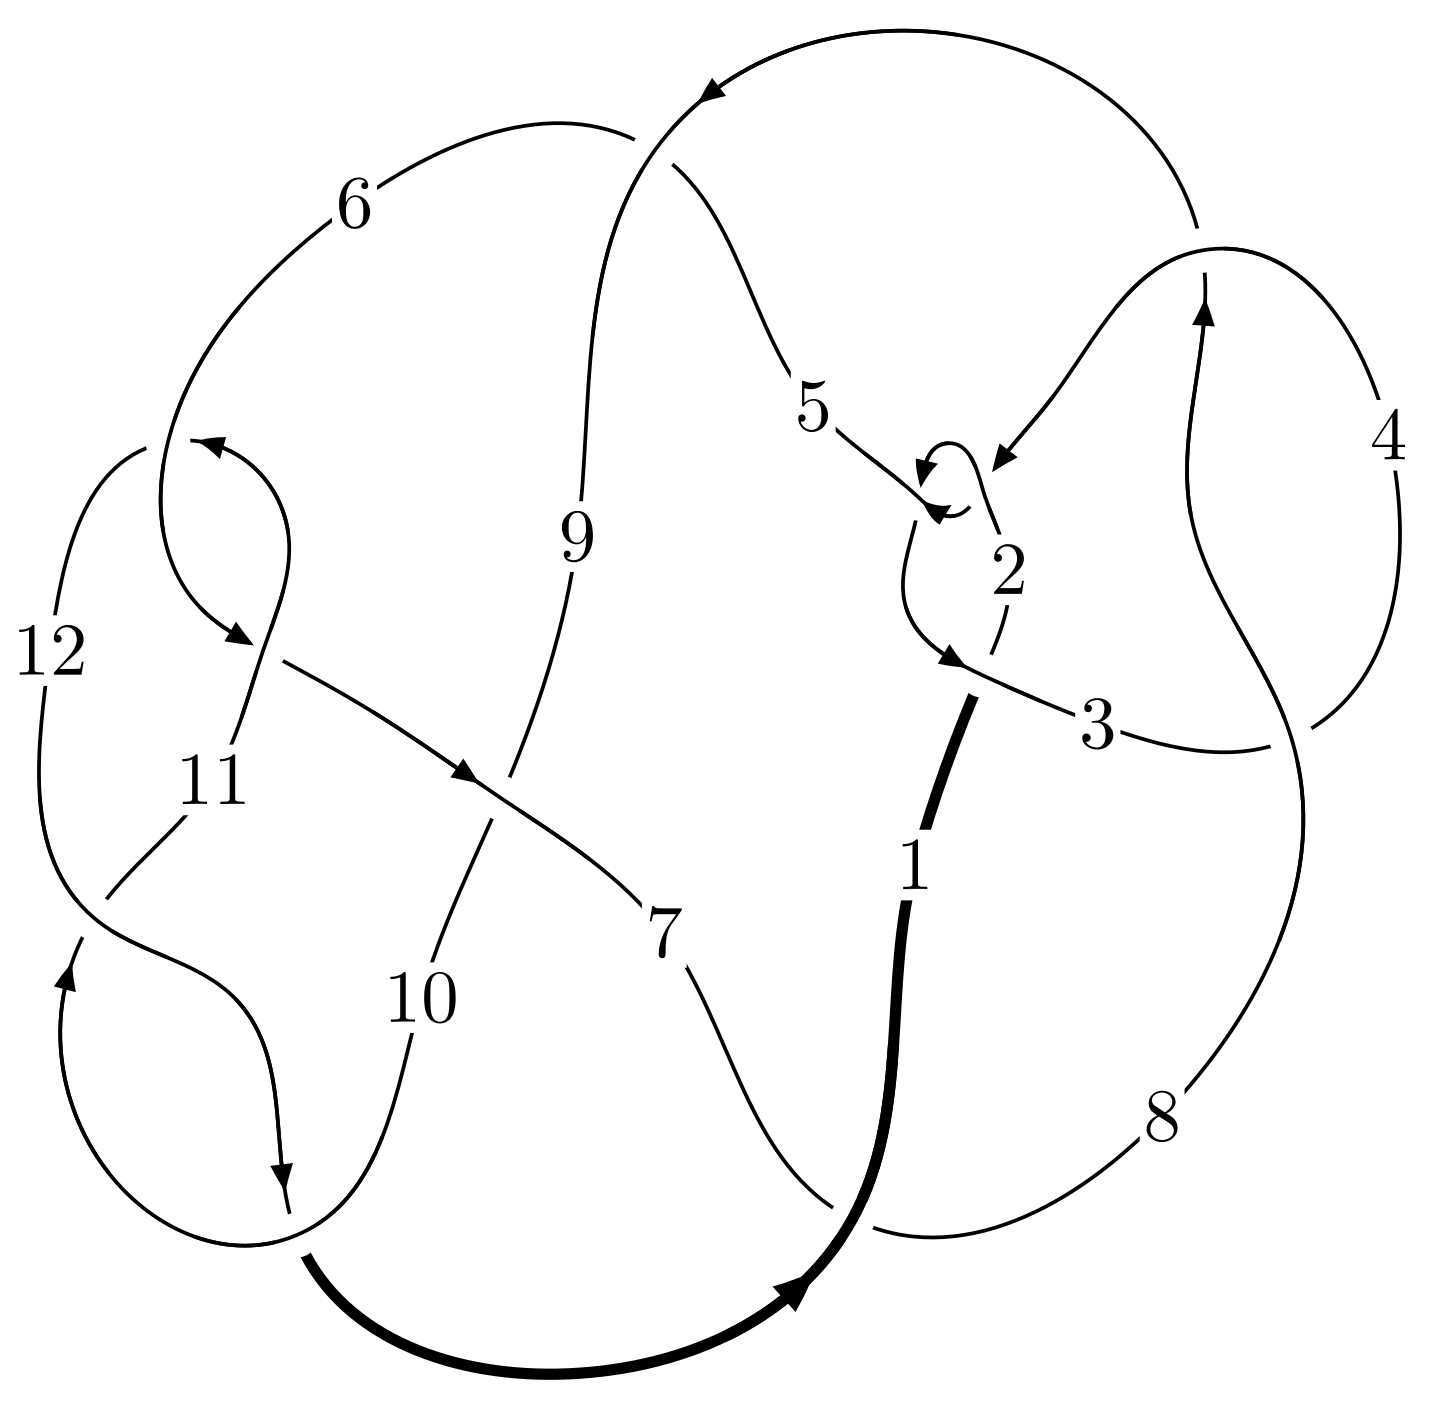
\includegraphics[width=112pt]{../../../GIT/diagram.site/Diagrams/png/888_12a_0087.png}\\
\ \ \ A knot diagram\footnotemark}&
\allowdisplaybreaks
\textbf{Linearized knot diagam} \\
\cline{2-2}
 &
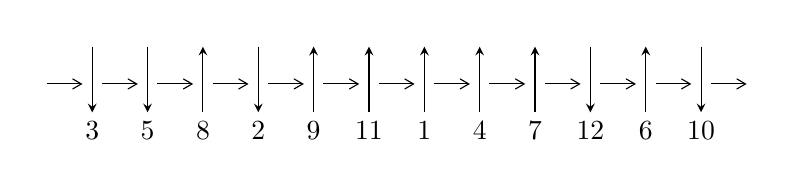
\begin{tikzpicture}[x=20pt, y=17pt]
	% nodes
	\node (C0) at (0, 0) {};
	\node (C1) at (1, 0) {};
	\node (C1U) at (1, +1) {};
	\node (C1D) at (1, -1) {3};

	\node (C2) at (2, 0) {};
	\node (C2U) at (2, +1) {};
	\node (C2D) at (2, -1) {5};

	\node (C3) at (3, 0) {};
	\node (C3U) at (3, +1) {};
	\node (C3D) at (3, -1) {8};

	\node (C4) at (4, 0) {};
	\node (C4U) at (4, +1) {};
	\node (C4D) at (4, -1) {2};

	\node (C5) at (5, 0) {};
	\node (C5U) at (5, +1) {};
	\node (C5D) at (5, -1) {9};

	\node (C6) at (6, 0) {};
	\node (C6U) at (6, +1) {};
	\node (C6D) at (6, -1) {11};

	\node (C7) at (7, 0) {};
	\node (C7U) at (7, +1) {};
	\node (C7D) at (7, -1) {1};

	\node (C8) at (8, 0) {};
	\node (C8U) at (8, +1) {};
	\node (C8D) at (8, -1) {4};

	\node (C9) at (9, 0) {};
	\node (C9U) at (9, +1) {};
	\node (C9D) at (9, -1) {7};

	\node (C10) at (10, 0) {};
	\node (C10U) at (10, +1) {};
	\node (C10D) at (10, -1) {12};

	\node (C11) at (11, 0) {};
	\node (C11U) at (11, +1) {};
	\node (C11D) at (11, -1) {6};

	\node (C12) at (12, 0) {};
	\node (C12U) at (12, +1) {};
	\node (C12D) at (12, -1) {10};
	\node (C13) at (13, 0) {};

	% arrows
	\draw[->,>={angle 60}]
	(C0) edge (C1) (C1) edge (C2) (C2) edge (C3) (C3) edge (C4) (C4) edge (C5) (C5) edge (C6) (C6) edge (C7) (C7) edge (C8) (C8) edge (C9) (C9) edge (C10) (C10) edge (C11) (C11) edge (C12) (C12) edge (C13) ;	\draw[->,>=stealth]
	(C1U) edge (C1D) (C2U) edge (C2D) (C3D) edge (C3U) (C4U) edge (C4D) (C5D) edge (C5U) (C6D) edge (C6U) (C7D) edge (C7U) (C8D) edge (C8U) (C9D) edge (C9U) (C10U) edge (C10D) (C11D) edge (C11U) (C12U) edge (C12D) ;
	\end{tikzpicture} \\
\hhline{~~} \\& 
\textbf{Solving Sequence} \\ \cline{2-2} 
 &
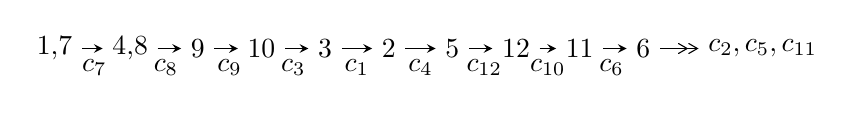
\begin{tikzpicture}[x=23pt, y=7pt]
	% node
	\node (A0) at (-1/8, 0) {1,7};
	\node (A1) at (17/16, 0) {4,8};
	\node (A2) at (17/8, 0) {9};
	\node (A3) at (25/8, 0) {10};
	\node (A4) at (33/8, 0) {3};
	\node (A5) at (41/8, 0) {2};
	\node (A6) at (49/8, 0) {5};
	\node (A7) at (57/8, 0) {12};
	\node (A8) at (65/8, 0) {11};
	\node (A9) at (73/8, 0) {6};
	\node (C1) at (1/2, -1) {$c_{7}$};
	\node (C2) at (13/8, -1) {$c_{8}$};
	\node (C3) at (21/8, -1) {$c_{9}$};
	\node (C4) at (29/8, -1) {$c_{3}$};
	\node (C5) at (37/8, -1) {$c_{1}$};
	\node (C6) at (45/8, -1) {$c_{4}$};
	\node (C7) at (53/8, -1) {$c_{12}$};
	\node (C8) at (61/8, -1) {$c_{10}$};
	\node (C9) at (69/8, -1) {$c_{6}$};
	\node (A10) at (11, 0) {$c_{2},c_{5},c_{11}$};

	% edge
	\draw[->,>=stealth]	
	(A0) edge (A1) (A1) edge (A2) (A2) edge (A3) (A3) edge (A4) (A4) edge (A5) (A5) edge (A6) (A6) edge (A7) (A7) edge (A8) (A8) edge (A9) ;
	\draw[->>,>={angle 60}]	
	(A9) edge (A10);
\end{tikzpicture} \\ 

\end{tabular} \\

\footnotetext{
The image of knot diagram is generated by the software ``\textbf{Draw programme}" developed by Andrew Bartholomew(\url{http://www.layer8.co.uk/maths/draw/index.htm\#Running-draw}), where we modified some parts for our purpose(\url{https://github.com/CATsTAILs/LinksPainter}).
}\phantom \\ \newline 
\centering \textbf{Ideals for irreducible components\footnotemark of $X_{\text{par}}$} 
 
\begin{align*}
I^u_{1}&=\langle 
1.26080\times10^{259} u^{95}+6.13882\times10^{258} u^{94}+\cdots+2.17742\times10^{262} b+1.97351\times10^{262},\\
\phantom{I^u_{1}}&\phantom{= \langle  }-1.46854\times10^{260} u^{95}+1.49274\times10^{260} u^{94}+\cdots+1.08871\times10^{263} a-6.09536\times10^{263},\\
\phantom{I^u_{1}}&\phantom{= \langle  }u^{96}-2 u^{95}+\cdots-460 u-200\rangle \\
I^u_{2}&=\langle 
b- u,\;- u^8+u^7+2 u^6-3 u^5- u^4+3 u^3-2 u^2+a+1,\;u^9- u^8-2 u^7+3 u^6+u^5-3 u^4+2 u^3- u+1\rangle \\
\\
\end{align*}
\raggedright * 2 irreducible components of $\dim_{\mathbb{C}}=0$, with total 105 representations.\\
\footnotetext{All coefficients of polynomials are rational numbers. But the coefficients are sometimes approximated in decimal forms when there is not enough margin.}
\newpage
\renewcommand{\arraystretch}{1}
\centering \section*{I. $I^u_{1}= \langle 1.26\times10^{259} u^{95}+6.14\times10^{258} u^{94}+\cdots+2.18\times10^{262} b+1.97\times10^{262},\;-1.47\times10^{260} u^{95}+1.49\times10^{260} u^{94}+\cdots+1.09\times10^{263} a-6.10\times10^{263},\;u^{96}-2 u^{95}+\cdots-460 u-200 \rangle$}
\flushleft \textbf{(i) Arc colorings}\\
\begin{tabular}{m{7pt} m{180pt} m{7pt} m{180pt} }
\flushright $a_{1}=$&$\begin{pmatrix}0\\u\end{pmatrix}$ \\
\flushright $a_{7}=$&$\begin{pmatrix}1\\0\end{pmatrix}$ \\
\flushright $a_{4}=$&$\begin{pmatrix}0.00134888 u^{95}-0.00137111 u^{94}+\cdots-23.9339 u+5.59870\\-0.000579033 u^{95}-0.000281931 u^{94}+\cdots+1.99179 u-0.906349\end{pmatrix}$ \\
\flushright $a_{8}=$&$\begin{pmatrix}1\\- u^2\end{pmatrix}$ \\
\flushright $a_{9}=$&$\begin{pmatrix}-0.00264479 u^{95}+0.00389553 u^{94}+\cdots-21.5177 u+8.21684\\-0.00108988 u^{95}+0.000477782 u^{94}+\cdots-2.75847 u-1.78684\end{pmatrix}$ \\
\flushright $a_{10}=$&$\begin{pmatrix}-0.00373468 u^{95}+0.00437331 u^{94}+\cdots-24.2761 u+6.43000\\-0.00108988 u^{95}+0.000477782 u^{94}+\cdots-2.75847 u-1.78684\end{pmatrix}$ \\
\flushright $a_{3}=$&$\begin{pmatrix}-0.000268801 u^{95}+0.000972032 u^{94}+\cdots-26.8057 u+6.23972\\0.000223594 u^{95}-0.00110886 u^{94}+\cdots+2.72574 u-0.727907\end{pmatrix}$ \\
\flushright $a_{2}=$&$\begin{pmatrix}0.00893103 u^{95}-0.0164647 u^{94}+\cdots-30.2478 u-0.173459\\-0.000308624 u^{95}+0.00120035 u^{94}+\cdots+7.65580 u-0.365428\end{pmatrix}$ \\
\flushright $a_{5}=$&$\begin{pmatrix}0.0103283 u^{95}-0.0184415 u^{94}+\cdots-30.8959 u-0.822307\\-0.00139406 u^{95}+0.00166301 u^{94}+\cdots+7.00023 u-0.528959\end{pmatrix}$ \\
\flushright $a_{12}=$&$\begin{pmatrix}-0.00735718 u^{95}+0.0171983 u^{94}+\cdots+35.3516 u+1.21405\\-0.00106631 u^{95}-0.000829870 u^{94}+\cdots-8.00807 u+0.599583\end{pmatrix}$ \\
\flushright $a_{11}=$&$\begin{pmatrix}0.00580303 u^{95}-0.0104224 u^{94}+\cdots+4.52281 u-6.13898\\0.000466017 u^{95}+0.000741362 u^{94}+\cdots+4.55819 u+0.807933\end{pmatrix}$ \\
\flushright $a_{6}=$&$\begin{pmatrix}0.00893420 u^{95}-0.0167785 u^{94}+\cdots-23.8956 u-1.35127\\-0.00309604 u^{95}+0.00328517 u^{94}+\cdots+4.71205 u-0.746936\end{pmatrix}$\\&\end{tabular}
\flushleft \textbf{(ii) Obstruction class $= -1$}\\~\\
\flushleft \textbf{(iii) Cusp Shapes $= 0.00392468 u^{95}-0.00398262 u^{94}+\cdots-17.9482 u+11.0656$}\\~\\
\newpage\renewcommand{\arraystretch}{1}
\flushleft \textbf{(iv) u-Polynomials at the component}\newline \\
\begin{tabular}{m{50pt}|m{274pt}}
Crossings & \hspace{64pt}u-Polynomials at each crossing \\
\hline $$\begin{aligned}c_{1}\end{aligned}$$&$\begin{aligned}
&u^{96}+42 u^{95}+\cdots+29 u+1
\end{aligned}$\\
\hline $$\begin{aligned}c_{2},c_{4}\end{aligned}$$&$\begin{aligned}
&u^{96}-10 u^{95}+\cdots+13 u-1
\end{aligned}$\\
\hline $$\begin{aligned}c_{3},c_{8}\end{aligned}$$&$\begin{aligned}
&u^{96}+u^{95}+\cdots+1536 u+512
\end{aligned}$\\
\hline $$\begin{aligned}c_{5},c_{7}\end{aligned}$$&$\begin{aligned}
&u^{96}-2 u^{95}+\cdots-460 u-200
\end{aligned}$\\
\hline $$\begin{aligned}c_{6},c_{11}\end{aligned}$$&$\begin{aligned}
&u^{96}-2 u^{95}+\cdots+u-1
\end{aligned}$\\
\hline $$\begin{aligned}c_{9}\end{aligned}$$&$\begin{aligned}
&u^{96}+10 u^{95}+\cdots-45760 u-5824
\end{aligned}$\\
\hline $$\begin{aligned}c_{10},c_{12}\end{aligned}$$&$\begin{aligned}
&u^{96}+30 u^{95}+\cdots+7 u+1
\end{aligned}$\\
\hline
\end{tabular}\\~\\
\newpage\renewcommand{\arraystretch}{1}
\flushleft \textbf{(v) Riley Polynomials at the component}\newline \\
\begin{tabular}{m{50pt}|m{274pt}}
Crossings & \hspace{64pt}Riley Polynomials at each crossing \\
\hline $$\begin{aligned}c_{1}\end{aligned}$$&$\begin{aligned}
&y^{96}+34 y^{95}+\cdots-261 y+1
\end{aligned}$\\
\hline $$\begin{aligned}c_{2},c_{4}\end{aligned}$$&$\begin{aligned}
&y^{96}-42 y^{95}+\cdots-29 y+1
\end{aligned}$\\
\hline $$\begin{aligned}c_{3},c_{8}\end{aligned}$$&$\begin{aligned}
&y^{96}-57 y^{95}+\cdots-7602176 y+262144
\end{aligned}$\\
\hline $$\begin{aligned}c_{5},c_{7}\end{aligned}$$&$\begin{aligned}
&y^{96}-82 y^{95}+\cdots+739600 y+40000
\end{aligned}$\\
\hline $$\begin{aligned}c_{6},c_{11}\end{aligned}$$&$\begin{aligned}
&y^{96}+30 y^{95}+\cdots+7 y+1
\end{aligned}$\\
\hline $$\begin{aligned}c_{9}\end{aligned}$$&$\begin{aligned}
&y^{96}-26 y^{95}+\cdots+1172319616 y+33918976
\end{aligned}$\\
\hline $$\begin{aligned}c_{10},c_{12}\end{aligned}$$&$\begin{aligned}
&y^{96}+74 y^{95}+\cdots+79 y+1
\end{aligned}$\\
\hline
\end{tabular}\\~\\
\newpage\flushleft \textbf{(vi) Complex Volumes and Cusp Shapes}
$$\begin{array}{c|c|c}  
\text{Solutions to }I^u_{1}& \I (\text{vol} + \sqrt{-1}CS) & \text{Cusp shape}\\
 \hline 
\begin{aligned}
u &= \phantom{-}0.827779 + 0.624593 I \\
a &= \phantom{-}0.766054 - 0.164191 I \\
b &= \phantom{-}0.493580 - 0.463043 I\end{aligned}
 & \phantom{-}3.48652 + 0.96941 I & \phantom{-0.000000 } 0 \\ \hline\begin{aligned}
u &= \phantom{-}0.827779 - 0.624593 I \\
a &= \phantom{-}0.766054 + 0.164191 I \\
b &= \phantom{-}0.493580 + 0.463043 I\end{aligned}
 & \phantom{-}3.48652 - 0.96941 I & \phantom{-0.000000 } 0 \\ \hline\begin{aligned}
u &= -0.776180 + 0.705899 I \\
a &= -0.791059 - 0.015213 I \\
b &= -0.729017 - 0.490853 I\end{aligned}
 & \phantom{-}2.73740 - 6.45315 I & \phantom{-0.000000 } 0 \\ \hline\begin{aligned}
u &= -0.776180 - 0.705899 I \\
a &= -0.791059 + 0.015213 I \\
b &= -0.729017 + 0.490853 I\end{aligned}
 & \phantom{-}2.73740 + 6.45315 I & \phantom{-0.000000 } 0 \\ \hline\begin{aligned}
u &= \phantom{-}0.464918 + 0.808617 I \\
a &= \phantom{-}0.742252 + 0.500605 I \\
b &= \phantom{-}1.20591 - 1.12994 I\end{aligned}
 & -1.02113 + 6.02463 I & \phantom{-0.000000 } 0. - 6.77260 I \\ \hline\begin{aligned}
u &= \phantom{-}0.464918 - 0.808617 I \\
a &= \phantom{-}0.742252 - 0.500605 I \\
b &= \phantom{-}1.20591 + 1.12994 I\end{aligned}
 & -1.02113 - 6.02463 I & \phantom{-0.000000 -}0. + 6.77260 I \\ \hline\begin{aligned}
u &= -0.378156 + 1.002420 I \\
a &= -0.0671290 - 0.0699448 I \\
b &= -0.934967 - 0.347321 I\end{aligned}
 & -0.05564 + 4.08075 I & \phantom{-0.000000 } 0 \\ \hline\begin{aligned}
u &= -0.378156 - 1.002420 I \\
a &= -0.0671290 + 0.0699448 I \\
b &= -0.934967 + 0.347321 I\end{aligned}
 & -0.05564 - 4.08075 I & \phantom{-0.000000 } 0 \\ \hline\begin{aligned}
u &= -1.100440 + 0.034710 I \\
a &= \phantom{-}0.158113 + 0.235477 I \\
b &= -0.364706 + 0.755399 I\end{aligned}
 & -0.475309 - 0.554742 I & \phantom{-0.000000 } 0 \\ \hline\begin{aligned}
u &= -1.100440 - 0.034710 I \\
a &= \phantom{-}0.158113 - 0.235477 I \\
b &= -0.364706 - 0.755399 I\end{aligned}
 & -0.475309 + 0.554742 I & \phantom{-0.000000 } 0\\
 \hline 
 \end{array}$$\newpage$$\begin{array}{c|c|c}  
\text{Solutions to }I^u_{1}& \I (\text{vol} + \sqrt{-1}CS) & \text{Cusp shape}\\
 \hline 
\begin{aligned}
u &= \phantom{-}0.198330 + 0.838237 I \\
a &= -0.004574 + 0.568131 I \\
b &= -0.892057 + 0.019153 I\end{aligned}
 & \phantom{-}0.69375 + 4.11299 I & \phantom{-}4.80660 - 6.49721 I \\ \hline\begin{aligned}
u &= \phantom{-}0.198330 - 0.838237 I \\
a &= -0.004574 - 0.568131 I \\
b &= -0.892057 - 0.019153 I\end{aligned}
 & \phantom{-}0.69375 - 4.11299 I & \phantom{-}4.80660 + 6.49721 I \\ \hline\begin{aligned}
u &= \phantom{-}0.566068 + 0.648047 I \\
a &= \phantom{-}0.125153 - 0.466570 I \\
b &= \phantom{-}0.658996 - 0.216976 I\end{aligned}
 & \phantom{-}1.40639 - 0.40707 I & \phantom{-}7.71113 + 0. I\phantom{ +0.000000I} \\ \hline\begin{aligned}
u &= \phantom{-}0.566068 - 0.648047 I \\
a &= \phantom{-}0.125153 + 0.466570 I \\
b &= \phantom{-}0.658996 + 0.216976 I\end{aligned}
 & \phantom{-}1.40639 + 0.40707 I & \phantom{-}7.71113 + 0. I\phantom{ +0.000000I} \\ \hline\begin{aligned}
u &= \phantom{-}1.123300 + 0.256960 I \\
a &= -2.35906 + 0.10801 I \\
b &= \phantom{-}1.95563 + 1.12656 I\end{aligned}
 & -2.14141 + 2.71496 I & \phantom{-0.000000 } 0 \\ \hline\begin{aligned}
u &= \phantom{-}1.123300 - 0.256960 I \\
a &= -2.35906 - 0.10801 I \\
b &= \phantom{-}1.95563 - 1.12656 I\end{aligned}
 & -2.14141 - 2.71496 I & \phantom{-0.000000 } 0 \\ \hline\begin{aligned}
u &= -0.536243 + 0.654347 I \\
a &= -0.505424 + 0.534295 I \\
b &= -0.879070 - 1.082410 I\end{aligned}
 & -0.382139 - 0.796657 I & \phantom{-}1.13878 + 1.64523 I \\ \hline\begin{aligned}
u &= -0.536243 - 0.654347 I \\
a &= -0.505424 - 0.534295 I \\
b &= -0.879070 + 1.082410 I\end{aligned}
 & -0.382139 + 0.796657 I & \phantom{-}1.13878 - 1.64523 I \\ \hline\begin{aligned}
u &= -0.026316 + 1.166270 I \\
a &= \phantom{-}0.175568 + 0.203349 I \\
b &= \phantom{-}1.195080 - 0.079544 I\end{aligned}
 & -0.448862 + 0.214466 I & \phantom{-0.000000 } 0 \\ \hline\begin{aligned}
u &= -0.026316 - 1.166270 I \\
a &= \phantom{-}0.175568 - 0.203349 I \\
b &= \phantom{-}1.195080 + 0.079544 I\end{aligned}
 & -0.448862 - 0.214466 I & \phantom{-0.000000 } 0\\
 \hline 
 \end{array}$$\newpage$$\begin{array}{c|c|c}  
\text{Solutions to }I^u_{1}& \I (\text{vol} + \sqrt{-1}CS) & \text{Cusp shape}\\
 \hline 
\begin{aligned}
u &= -0.274505 + 0.786774 I \\
a &= \phantom{-}1.76746 + 0.75543 I \\
b &= \phantom{-}1.30709 + 0.68152 I\end{aligned}
 & -1.42380 - 3.79251 I & \phantom{-0.000000 -}0. + 7.12596 I \\ \hline\begin{aligned}
u &= -0.274505 - 0.786774 I \\
a &= \phantom{-}1.76746 - 0.75543 I \\
b &= \phantom{-}1.30709 - 0.68152 I\end{aligned}
 & -1.42380 + 3.79251 I & \phantom{-0.000000 } 0. - 7.12596 I \\ \hline\begin{aligned}
u &= \phantom{-}0.711183 + 0.933780 I \\
a &= -0.664766 + 0.629968 I \\
b &= -0.525651 + 0.615669 I\end{aligned}
 & \phantom{-}1.83320 + 5.67791 I & \phantom{-0.000000 } 0 \\ \hline\begin{aligned}
u &= \phantom{-}0.711183 - 0.933780 I \\
a &= -0.664766 - 0.629968 I \\
b &= -0.525651 - 0.615669 I\end{aligned}
 & \phantom{-}1.83320 - 5.67791 I & \phantom{-0.000000 } 0 \\ \hline\begin{aligned}
u &= -0.813850 + 0.858127 I \\
a &= -0.267229 - 0.194580 I \\
b &= -0.572924 - 0.483599 I\end{aligned}
 & -2.36574 - 1.38104 I & \phantom{-0.000000 } 0 \\ \hline\begin{aligned}
u &= -0.813850 - 0.858127 I \\
a &= -0.267229 + 0.194580 I \\
b &= -0.572924 + 0.483599 I\end{aligned}
 & -2.36574 + 1.38104 I & \phantom{-0.000000 } 0 \\ \hline\begin{aligned}
u &= \phantom{-}0.113824 + 0.777555 I \\
a &= \phantom{-}1.15581 + 0.83439 I \\
b &= \phantom{-}1.38543 - 0.35114 I\end{aligned}
 & -5.10467 + 1.06897 I & -7.34001 - 0.30204 I \\ \hline\begin{aligned}
u &= \phantom{-}0.113824 - 0.777555 I \\
a &= \phantom{-}1.15581 - 0.83439 I \\
b &= \phantom{-}1.38543 + 0.35114 I\end{aligned}
 & -5.10467 - 1.06897 I & -7.34001 + 0.30204 I \\ \hline\begin{aligned}
u &= -1.21618\phantom{ +0.000000I} \\
a &= \phantom{-}2.35855\phantom{ +0.000000I} \\
b &= -2.53045\phantom{ +0.000000I}\end{aligned}
 & \phantom{-}0.969248\phantom{ +0.000000I} & \phantom{-0.000000 } 0 \\ \hline\begin{aligned}
u &= \phantom{-}1.093860 + 0.533224 I \\
a &= \phantom{-}0.368064 - 0.089389 I \\
b &= \phantom{-}0.248387 - 0.349717 I\end{aligned}
 & \phantom{-}3.61901 + 1.02354 I & \phantom{-0.000000 } 0\\
 \hline 
 \end{array}$$\newpage$$\begin{array}{c|c|c}  
\text{Solutions to }I^u_{1}& \I (\text{vol} + \sqrt{-1}CS) & \text{Cusp shape}\\
 \hline 
\begin{aligned}
u &= \phantom{-}1.093860 - 0.533224 I \\
a &= \phantom{-}0.368064 + 0.089389 I \\
b &= \phantom{-}0.248387 + 0.349717 I\end{aligned}
 & \phantom{-}3.61901 - 1.02354 I & \phantom{-0.000000 } 0 \\ \hline\begin{aligned}
u &= -0.423602 + 1.151240 I \\
a &= \phantom{-}0.408811 + 0.403769 I \\
b &= \phantom{-}1.106640 + 0.403349 I\end{aligned}
 & -3.57664 - 5.39810 I & \phantom{-0.000000 } 0 \\ \hline\begin{aligned}
u &= -0.423602 - 1.151240 I \\
a &= \phantom{-}0.408811 - 0.403769 I \\
b &= \phantom{-}1.106640 - 0.403349 I\end{aligned}
 & -3.57664 + 5.39810 I & \phantom{-0.000000 } 0 \\ \hline\begin{aligned}
u &= \phantom{-}0.400539 + 0.627675 I \\
a &= -2.07511 + 0.80787 I \\
b &= -0.747446 + 0.842065 I\end{aligned}
 & -0.95421 - 1.31729 I & \phantom{-}2.18400 - 2.06346 I \\ \hline\begin{aligned}
u &= \phantom{-}0.400539 - 0.627675 I \\
a &= -2.07511 - 0.80787 I \\
b &= -0.747446 - 0.842065 I\end{aligned}
 & -0.95421 + 1.31729 I & \phantom{-}2.18400 + 2.06346 I \\ \hline\begin{aligned}
u &= -0.445856 + 0.557895 I \\
a &= -0.544443 + 0.185637 I \\
b &= -0.673309 + 0.120518 I\end{aligned}
 & -2.01713 - 1.57713 I & \phantom{-}0.42883 + 4.65454 I \\ \hline\begin{aligned}
u &= -0.445856 - 0.557895 I \\
a &= -0.544443 - 0.185637 I \\
b &= -0.673309 - 0.120518 I\end{aligned}
 & -2.01713 + 1.57713 I & \phantom{-}0.42883 - 4.65454 I \\ \hline\begin{aligned}
u &= \phantom{-}1.286230 + 0.076999 I \\
a &= -1.80122 + 0.72733 I \\
b &= \phantom{-}1.74533 - 1.39516 I\end{aligned}
 & \phantom{-}9.63218 + 0.67885 I & \phantom{-0.000000 } 0 \\ \hline\begin{aligned}
u &= \phantom{-}1.286230 - 0.076999 I \\
a &= -1.80122 - 0.72733 I \\
b &= \phantom{-}1.74533 + 1.39516 I\end{aligned}
 & \phantom{-}9.63218 - 0.67885 I & \phantom{-0.000000 } 0 \\ \hline\begin{aligned}
u &= \phantom{-}1.234880 + 0.379536 I \\
a &= -1.48139 + 0.72164 I \\
b &= \phantom{-}1.42509 - 0.17205 I\end{aligned}
 & \phantom{-}3.11379 + 5.16324 I & \phantom{-0.000000 } 0\\
 \hline 
 \end{array}$$\newpage$$\begin{array}{c|c|c}  
\text{Solutions to }I^u_{1}& \I (\text{vol} + \sqrt{-1}CS) & \text{Cusp shape}\\
 \hline 
\begin{aligned}
u &= \phantom{-}1.234880 - 0.379536 I \\
a &= -1.48139 - 0.72164 I \\
b &= \phantom{-}1.42509 + 0.17205 I\end{aligned}
 & \phantom{-}3.11379 - 5.16324 I & \phantom{-0.000000 } 0 \\ \hline\begin{aligned}
u &= \phantom{-}1.289470 + 0.129396 I \\
a &= \phantom{-}0.014621 - 0.284789 I \\
b &= \phantom{-}0.103192 - 0.622026 I\end{aligned}
 & \phantom{-}2.48955 + 2.34627 I & \phantom{-0.000000 } 0 \\ \hline\begin{aligned}
u &= \phantom{-}1.289470 - 0.129396 I \\
a &= \phantom{-}0.014621 + 0.284789 I \\
b &= \phantom{-}0.103192 + 0.622026 I\end{aligned}
 & \phantom{-}2.48955 - 2.34627 I & \phantom{-0.000000 } 0 \\ \hline\begin{aligned}
u &= -1.274750 + 0.328982 I \\
a &= -0.139931 - 0.224618 I \\
b &= \phantom{-}0.111267 - 0.851993 I\end{aligned}
 & -0.81320 - 5.10776 I & \phantom{-0.000000 } 0 \\ \hline\begin{aligned}
u &= -1.274750 - 0.328982 I \\
a &= -0.139931 + 0.224618 I \\
b &= \phantom{-}0.111267 + 0.851993 I\end{aligned}
 & -0.81320 + 5.10776 I & \phantom{-0.000000 } 0 \\ \hline\begin{aligned}
u &= \phantom{-}1.310800 + 0.170091 I \\
a &= \phantom{-}1.62551 - 0.47736 I \\
b &= -1.61937 + 0.38777 I\end{aligned}
 & \phantom{-}4.79007 - 0.70146 I & \phantom{-0.000000 } 0 \\ \hline\begin{aligned}
u &= \phantom{-}1.310800 - 0.170091 I \\
a &= \phantom{-}1.62551 + 0.47736 I \\
b &= -1.61937 - 0.38777 I\end{aligned}
 & \phantom{-}4.79007 + 0.70146 I & \phantom{-0.000000 } 0 \\ \hline\begin{aligned}
u &= -0.745639 + 1.091740 I \\
a &= \phantom{-}0.674140 + 0.477527 I \\
b &= \phantom{-}0.737945 + 0.876759 I\end{aligned}
 & \phantom{-}0.85649 - 10.99580 I & \phantom{-0.000000 } 0 \\ \hline\begin{aligned}
u &= -0.745639 - 1.091740 I \\
a &= \phantom{-}0.674140 - 0.477527 I \\
b &= \phantom{-}0.737945 - 0.876759 I\end{aligned}
 & \phantom{-}0.85649 + 10.99580 I & \phantom{-0.000000 } 0 \\ \hline\begin{aligned}
u &= -1.140160 + 0.671129 I \\
a &= -0.338273 - 0.104862 I \\
b &= -0.253242 - 0.467981 I\end{aligned}
 & \phantom{-}2.79217 - 6.69642 I & \phantom{-0.000000 } 0\\
 \hline 
 \end{array}$$\newpage$$\begin{array}{c|c|c}  
\text{Solutions to }I^u_{1}& \I (\text{vol} + \sqrt{-1}CS) & \text{Cusp shape}\\
 \hline 
\begin{aligned}
u &= -1.140160 - 0.671129 I \\
a &= -0.338273 + 0.104862 I \\
b &= -0.253242 + 0.467981 I\end{aligned}
 & \phantom{-}2.79217 + 6.69642 I & \phantom{-0.000000 } 0 \\ \hline\begin{aligned}
u &= -1.342110 + 0.110731 I \\
a &= \phantom{-}1.76836 + 0.67077 I \\
b &= -1.99856 - 1.24201 I\end{aligned}
 & \phantom{-}10.26590 - 6.65314 I & \phantom{-0.000000 } 0 \\ \hline\begin{aligned}
u &= -1.342110 - 0.110731 I \\
a &= \phantom{-}1.76836 - 0.67077 I \\
b &= -1.99856 + 1.24201 I\end{aligned}
 & \phantom{-}10.26590 + 6.65314 I & \phantom{-0.000000 } 0 \\ \hline\begin{aligned}
u &= -1.346640 + 0.193829 I \\
a &= \phantom{-}0.133789 + 0.425172 I \\
b &= -0.577467 + 0.438500 I\end{aligned}
 & \phantom{-}5.59084 - 5.35666 I & \phantom{-0.000000 } 0 \\ \hline\begin{aligned}
u &= -1.346640 - 0.193829 I \\
a &= \phantom{-}0.133789 - 0.425172 I \\
b &= -0.577467 - 0.438500 I\end{aligned}
 & \phantom{-}5.59084 + 5.35666 I & \phantom{-0.000000 } 0 \\ \hline\begin{aligned}
u &= \phantom{-}1.370410 + 0.134173 I \\
a &= -0.098663 + 0.414795 I \\
b &= \phantom{-}0.475158 + 0.391928 I\end{aligned}
 & \phantom{-}6.31687 - 0.55010 I & \phantom{-0.000000 } 0 \\ \hline\begin{aligned}
u &= \phantom{-}1.370410 - 0.134173 I \\
a &= -0.098663 - 0.414795 I \\
b &= \phantom{-}0.475158 - 0.391928 I\end{aligned}
 & \phantom{-}6.31687 + 0.55010 I & \phantom{-0.000000 } 0 \\ \hline\begin{aligned}
u &= \phantom{-}1.403460 + 0.020491 I \\
a &= \phantom{-}1.82408 + 0.48228 I \\
b &= -2.14446 - 1.34593 I\end{aligned}
 & \phantom{-}11.20810 + 5.45907 I & \phantom{-0.000000 } 0 \\ \hline\begin{aligned}
u &= \phantom{-}1.403460 - 0.020491 I \\
a &= \phantom{-}1.82408 - 0.48228 I \\
b &= -2.14446 + 1.34593 I\end{aligned}
 & \phantom{-}11.20810 - 5.45907 I & \phantom{-0.000000 } 0 \\ \hline\begin{aligned}
u &= \phantom{-}0.596086\phantom{ +0.000000I} \\
a &= \phantom{-}0.378856\phantom{ +0.000000I} \\
b &= \phantom{-}0.339787\phantom{ +0.000000I}\end{aligned}
 & \phantom{-}0.826795\phantom{ +0.000000I} & \phantom{-}12.3850\phantom{ +0.000000I}\\
 \hline 
 \end{array}$$\newpage$$\begin{array}{c|c|c}  
\text{Solutions to }I^u_{1}& \I (\text{vol} + \sqrt{-1}CS) & \text{Cusp shape}\\
 \hline 
\begin{aligned}
u &= -1.39415 + 0.24042 I \\
a &= \phantom{-}2.29080 + 0.05093 I \\
b &= -3.32398 + 1.35225 I\end{aligned}
 & \phantom{-}4.56353 - 1.83741 I & \phantom{-0.000000 } 0 \\ \hline\begin{aligned}
u &= -1.39415 - 0.24042 I \\
a &= \phantom{-}2.29080 - 0.05093 I \\
b &= -3.32398 - 1.35225 I\end{aligned}
 & \phantom{-}4.56353 + 1.83741 I & \phantom{-0.000000 } 0 \\ \hline\begin{aligned}
u &= \phantom{-}0.064541 + 0.574239 I \\
a &= -0.546201 + 0.542337 I \\
b &= -0.368226 + 0.853562 I\end{aligned}
 & \phantom{-}1.09357 + 2.72804 I & \phantom{-}4.37287 - 1.66251 I \\ \hline\begin{aligned}
u &= \phantom{-}0.064541 - 0.574239 I \\
a &= -0.546201 - 0.542337 I \\
b &= -0.368226 - 0.853562 I\end{aligned}
 & \phantom{-}1.09357 - 2.72804 I & \phantom{-}4.37287 + 1.66251 I \\ \hline\begin{aligned}
u &= \phantom{-}1.38970 + 0.30493 I \\
a &= -2.28182 + 0.06308 I \\
b &= \phantom{-}3.21670 + 1.70719 I\end{aligned}
 & \phantom{-}3.79038 + 7.72330 I & \phantom{-0.000000 } 0 \\ \hline\begin{aligned}
u &= \phantom{-}1.38970 - 0.30493 I \\
a &= -2.28182 - 0.06308 I \\
b &= \phantom{-}3.21670 - 1.70719 I\end{aligned}
 & \phantom{-}3.79038 - 7.72330 I & \phantom{-0.000000 } 0 \\ \hline\begin{aligned}
u &= -1.43873 + 0.01362 I \\
a &= -1.80826 - 0.44328 I \\
b &= \phantom{-}2.34251 + 1.15556 I\end{aligned}
 & \phantom{-}11.90280 - 0.51570 I & \phantom{-0.000000 } 0 \\ \hline\begin{aligned}
u &= -1.43873 - 0.01362 I \\
a &= -1.80826 + 0.44328 I \\
b &= \phantom{-}2.34251 - 1.15556 I\end{aligned}
 & \phantom{-}11.90280 + 0.51570 I & \phantom{-0.000000 } 0 \\ \hline\begin{aligned}
u &= -1.45282 + 0.21004 I \\
a &= -1.67134 - 0.35027 I \\
b &= \phantom{-}2.30394 + 0.06403 I\end{aligned}
 & \phantom{-}7.80775 - 2.46616 I & \phantom{-0.000000 } 0 \\ \hline\begin{aligned}
u &= -1.45282 - 0.21004 I \\
a &= -1.67134 + 0.35027 I \\
b &= \phantom{-}2.30394 - 0.06403 I\end{aligned}
 & \phantom{-}7.80775 + 2.46616 I & \phantom{-0.000000 } 0\\
 \hline 
 \end{array}$$\newpage$$\begin{array}{c|c|c}  
\text{Solutions to }I^u_{1}& \I (\text{vol} + \sqrt{-1}CS) & \text{Cusp shape}\\
 \hline 
\begin{aligned}
u &= -1.42836 + 0.35491 I \\
a &= \phantom{-}1.56214 + 0.55704 I \\
b &= -2.23729 - 0.08696 I\end{aligned}
 & \phantom{-}5.97343 - 8.45094 I & \phantom{-0.000000 } 0 \\ \hline\begin{aligned}
u &= -1.42836 - 0.35491 I \\
a &= \phantom{-}1.56214 - 0.55704 I \\
b &= -2.23729 + 0.08696 I\end{aligned}
 & \phantom{-}5.97343 + 8.45094 I & \phantom{-0.000000 } 0 \\ \hline\begin{aligned}
u &= -0.227545 + 0.469775 I \\
a &= \phantom{-}0.669485 + 0.611296 I \\
b &= \phantom{-}0.109400 + 0.953333 I\end{aligned}
 & \phantom{-}1.25988 + 2.50075 I & \phantom{-}4.93074 - 4.35385 I \\ \hline\begin{aligned}
u &= -0.227545 - 0.469775 I \\
a &= \phantom{-}0.669485 - 0.611296 I \\
b &= \phantom{-}0.109400 - 0.953333 I\end{aligned}
 & \phantom{-}1.25988 - 2.50075 I & \phantom{-}4.93074 + 4.35385 I \\ \hline\begin{aligned}
u &= \phantom{-}1.47830 + 0.28430 I \\
a &= \phantom{-}0.150661 - 0.359583 I \\
b &= -0.340358 - 0.512654 I\end{aligned}
 & \phantom{-}6.00203 + 4.38225 I & \phantom{-0.000000 } 0 \\ \hline\begin{aligned}
u &= \phantom{-}1.47830 - 0.28430 I \\
a &= \phantom{-}0.150661 + 0.359583 I \\
b &= -0.340358 + 0.512654 I\end{aligned}
 & \phantom{-}6.00203 - 4.38225 I & \phantom{-0.000000 } 0 \\ \hline\begin{aligned}
u &= \phantom{-}1.46841 + 0.33425 I \\
a &= \phantom{-}1.60248 - 0.27369 I \\
b &= -2.21204 - 0.61429 I\end{aligned}
 & \phantom{-}4.35724 + 5.37503 I & \phantom{-0.000000 } 0 \\ \hline\begin{aligned}
u &= \phantom{-}1.46841 - 0.33425 I \\
a &= \phantom{-}1.60248 + 0.27369 I \\
b &= -2.21204 + 0.61429 I\end{aligned}
 & \phantom{-}4.35724 - 5.37503 I & \phantom{-0.000000 } 0 \\ \hline\begin{aligned}
u &= -1.48449 + 0.33794 I \\
a &= -0.182448 - 0.354150 I \\
b &= \phantom{-}0.440507 - 0.586608 I\end{aligned}
 & \phantom{-}5.19049 - 10.28900 I & \phantom{-0.000000 } 0 \\ \hline\begin{aligned}
u &= -1.48449 - 0.33794 I \\
a &= -0.182448 + 0.354150 I \\
b &= \phantom{-}0.440507 + 0.586608 I\end{aligned}
 & \phantom{-}5.19049 + 10.28900 I & \phantom{-0.000000 } 0\\
 \hline 
 \end{array}$$\newpage$$\begin{array}{c|c|c}  
\text{Solutions to }I^u_{1}& \I (\text{vol} + \sqrt{-1}CS) & \text{Cusp shape}\\
 \hline 
\begin{aligned}
u &= \phantom{-}1.49767 + 0.48896 I \\
a &= -1.47863 + 0.46783 I \\
b &= \phantom{-}2.35341 + 0.59797 I\end{aligned}
 & \phantom{-}2.38378 + 11.28690 I & \phantom{-0.000000 } 0 \\ \hline\begin{aligned}
u &= \phantom{-}1.49767 - 0.48896 I \\
a &= -1.47863 - 0.46783 I \\
b &= \phantom{-}2.35341 - 0.59797 I\end{aligned}
 & \phantom{-}2.38378 - 11.28690 I & \phantom{-0.000000 } 0 \\ \hline\begin{aligned}
u &= -1.60171 + 0.28748 I \\
a &= -1.69683 - 0.22396 I \\
b &= \phantom{-}3.03634 - 0.58541 I\end{aligned}
 & \phantom{-}11.35890 - 4.75367 I & \phantom{-0.000000 } 0 \\ \hline\begin{aligned}
u &= -1.60171 - 0.28748 I \\
a &= -1.69683 + 0.22396 I \\
b &= \phantom{-}3.03634 + 0.58541 I\end{aligned}
 & \phantom{-}11.35890 + 4.75367 I & \phantom{-0.000000 } 0 \\ \hline\begin{aligned}
u &= \phantom{-}1.61272 + 0.32466 I \\
a &= \phantom{-}1.68260 - 0.20082 I \\
b &= -3.03258 - 0.82668 I\end{aligned}
 & \phantom{-}10.5170 + 10.7052 I & \phantom{-0.000000 } 0 \\ \hline\begin{aligned}
u &= \phantom{-}1.61272 - 0.32466 I \\
a &= \phantom{-}1.68260 + 0.20082 I \\
b &= -3.03258 + 0.82668 I\end{aligned}
 & \phantom{-}10.5170 - 10.7052 I & \phantom{-0.000000 } 0 \\ \hline\begin{aligned}
u &= -1.62641 + 0.39035 I \\
a &= \phantom{-}1.57855 + 0.40202 I \\
b &= -3.11954 + 0.35306 I\end{aligned}
 & \phantom{-}9.3431 - 10.8284 I & \phantom{-0.000000 } 0 \\ \hline\begin{aligned}
u &= -1.62641 - 0.39035 I \\
a &= \phantom{-}1.57855 - 0.40202 I \\
b &= -3.11954 - 0.35306 I\end{aligned}
 & \phantom{-}9.3431 + 10.8284 I & \phantom{-0.000000 } 0 \\ \hline\begin{aligned}
u &= -0.109583 + 0.281441 I \\
a &= -0.28901 + 2.49262 I \\
b &= -0.446133 - 0.376732 I\end{aligned}
 & -1.66371 - 0.62726 I & -3.34444 + 1.32021 I \\ \hline\begin{aligned}
u &= -0.109583 - 0.281441 I \\
a &= -0.28901 - 2.49262 I \\
b &= -0.446133 + 0.376732 I\end{aligned}
 & -1.66371 + 0.62726 I & -3.34444 - 1.32021 I\\
 \hline 
 \end{array}$$\newpage$$\begin{array}{c|c|c}  
\text{Solutions to }I^u_{1}& \I (\text{vol} + \sqrt{-1}CS) & \text{Cusp shape}\\
 \hline 
\begin{aligned}
u &= \phantom{-}1.65178 + 0.42833 I \\
a &= -1.55828 + 0.37748 I \\
b &= \phantom{-}3.17967 + 0.58690 I\end{aligned}
 & \phantom{-}8.4581 + 16.7665 I & \phantom{-0.000000 } 0 \\ \hline\begin{aligned}
u &= \phantom{-}1.65178 - 0.42833 I \\
a &= -1.55828 - 0.37748 I \\
b &= \phantom{-}3.17967 - 0.58690 I\end{aligned}
 & \phantom{-}8.4581 - 16.7665 I & \phantom{-0.000000 } 0 \\ \hline\begin{aligned}
u &= \phantom{-}0.236161 + 0.122429 I \\
a &= -1.29570 - 3.83873 I \\
b &= \phantom{-}1.085450 + 0.089161 I\end{aligned}
 & \phantom{-}6.12820 + 0.12816 I & \phantom{-}9.44901 + 0.18719 I \\ \hline\begin{aligned}
u &= \phantom{-}0.236161 - 0.122429 I \\
a &= -1.29570 + 3.83873 I \\
b &= \phantom{-}1.085450 - 0.089161 I\end{aligned}
 & \phantom{-}6.12820 - 0.12816 I & \phantom{-}9.44901 - 0.18719 I \\ \hline\begin{aligned}
u &= -0.096047 + 0.122605 I \\
a &= \phantom{-}5.78359 - 3.98742 I \\
b &= -1.134920 - 0.077601 I\end{aligned}
 & \phantom{-}6.02935 + 5.60945 I & \phantom{-}9.08052 - 5.99594 I \\ \hline\begin{aligned}
u &= -0.096047 - 0.122605 I \\
a &= \phantom{-}5.78359 + 3.98742 I \\
b &= -1.134920 + 0.077601 I\end{aligned}
 & \phantom{-}6.02935 - 5.60945 I & \phantom{-}9.08052 + 5.99594 I\\
 \hline 
 \end{array}$$\newpage\newpage\renewcommand{\arraystretch}{1}
\centering \section*{II. $I^u_{2}= \langle b- u,\;- u^8+u^7+\cdots+a+1,\;u^9- u^8-2 u^7+3 u^6+u^5-3 u^4+2 u^3- u+1 \rangle$}
\flushleft \textbf{(i) Arc colorings}\\
\begin{tabular}{m{7pt} m{180pt} m{7pt} m{180pt} }
\flushright $a_{1}=$&$\begin{pmatrix}0\\u\end{pmatrix}$ \\
\flushright $a_{7}=$&$\begin{pmatrix}1\\0\end{pmatrix}$ \\
\flushright $a_{4}=$&$\begin{pmatrix}u^8- u^7-2 u^6+3 u^5+u^4-3 u^3+2 u^2-1\\u\end{pmatrix}$ \\
\flushright $a_{8}=$&$\begin{pmatrix}1\\- u^2\end{pmatrix}$ \\
\flushright $a_{9}=$&$\begin{pmatrix}1\\- u^2\end{pmatrix}$ \\
\flushright $a_{10}=$&$\begin{pmatrix}- u^2+1\\- u^2\end{pmatrix}$ \\
\flushright $a_{3}=$&$\begin{pmatrix}u^8- u^7-2 u^6+3 u^5+u^4-3 u^3+2 u^2-1\\u\end{pmatrix}$ \\
\flushright $a_{2}=$&$\begin{pmatrix}u^8- u^7-2 u^6+3 u^5+u^4-3 u^3+2 u^2-1\\2 u\end{pmatrix}$ \\
\flushright $a_{5}=$&$\begin{pmatrix}0\\- u\end{pmatrix}$ \\
\flushright $a_{12}=$&$\begin{pmatrix}u^5-2 u^3+u\\u^5- u^3+u\end{pmatrix}$ \\
\flushright $a_{11}=$&$\begin{pmatrix}- u^8+3 u^6-3 u^4+1\\- u^8+2 u^6-2 u^4\end{pmatrix}$ \\
\flushright $a_{6}=$&$\begin{pmatrix}- u\\u^3- u\end{pmatrix}$\\&\end{tabular}
\flushleft \textbf{(ii) Obstruction class $= 1$}\\~\\
\flushleft \textbf{(iii) Cusp Shapes $= u^8-4 u^7-3 u^6+9 u^5-10 u^3+2 u^2-2 u-3$}\\~\\
\newpage\renewcommand{\arraystretch}{1}
\flushleft \textbf{(iv) u-Polynomials at the component}\newline \\
\begin{tabular}{m{50pt}|m{274pt}}
Crossings & \hspace{64pt}u-Polynomials at each crossing \\
\hline $$\begin{aligned}c_{1},c_{2}\end{aligned}$$&$\begin{aligned}
&(u-1)^9
\end{aligned}$\\
\hline $$\begin{aligned}c_{3},c_{8}\end{aligned}$$&$\begin{aligned}
&u^9
\end{aligned}$\\
\hline $$\begin{aligned}c_{4}\end{aligned}$$&$\begin{aligned}
&(u+1)^9
\end{aligned}$\\
\hline $$\begin{aligned}c_{5},c_{7}\end{aligned}$$&$\begin{aligned}
&u^9- u^8-2 u^7+3 u^6+u^5-3 u^4+2 u^3- u+1
\end{aligned}$\\
\hline $$\begin{aligned}c_{6}\end{aligned}$$&$\begin{aligned}
&u^9- u^8+2 u^7- u^6+3 u^5- u^4+2 u^3+u+1
\end{aligned}$\\
\hline $$\begin{aligned}c_{9}\end{aligned}$$&$\begin{aligned}
&u^9-5 u^8+12 u^7-15 u^6+9 u^5+u^4-4 u^3+2 u^2+u-1
\end{aligned}$\\
\hline $$\begin{aligned}c_{10}\end{aligned}$$&$\begin{aligned}
&u^9-3 u^8+8 u^7-13 u^6+17 u^5-17 u^4+12 u^3-6 u^2+u+1
\end{aligned}$\\
\hline $$\begin{aligned}c_{11}\end{aligned}$$&$\begin{aligned}
&u^9+u^8+2 u^7+u^6+3 u^5+u^4+2 u^3+u-1
\end{aligned}$\\
\hline $$\begin{aligned}c_{12}\end{aligned}$$&$\begin{aligned}
&u^9+3 u^8+8 u^7+13 u^6+17 u^5+17 u^4+12 u^3+6 u^2+u-1
\end{aligned}$\\
\hline
\end{tabular}\\~\\
\newpage\renewcommand{\arraystretch}{1}
\flushleft \textbf{(v) Riley Polynomials at the component}\newline \\
\begin{tabular}{m{50pt}|m{274pt}}
Crossings & \hspace{64pt}Riley Polynomials at each crossing \\
\hline $$\begin{aligned}c_{1},c_{2},c_{4}\end{aligned}$$&$\begin{aligned}
&(y-1)^9
\end{aligned}$\\
\hline $$\begin{aligned}c_{3},c_{8}\end{aligned}$$&$\begin{aligned}
&y^9
\end{aligned}$\\
\hline $$\begin{aligned}c_{5},c_{7}\end{aligned}$$&$\begin{aligned}
&y^9-5 y^8+12 y^7-15 y^6+9 y^5+y^4-4 y^3+2 y^2+y-1
\end{aligned}$\\
\hline $$\begin{aligned}c_{6},c_{11}\end{aligned}$$&$\begin{aligned}
&y^9+3 y^8+8 y^7+13 y^6+17 y^5+17 y^4+12 y^3+6 y^2+y-1
\end{aligned}$\\
\hline $$\begin{aligned}c_{9}\end{aligned}$$&$\begin{aligned}
&y^9- y^8+12 y^7-7 y^6+37 y^5+y^4-10 y^2+5 y-1
\end{aligned}$\\
\hline $$\begin{aligned}c_{10},c_{12}\end{aligned}$$&$\begin{aligned}
&y^9+7 y^8+20 y^7+25 y^6+5 y^5-15 y^4+22 y^2+13 y-1
\end{aligned}$\\
\hline
\end{tabular}\\~\\
\newpage\flushleft \textbf{(vi) Complex Volumes and Cusp Shapes}
$$\begin{array}{c|c|c}  
\text{Solutions to }I^u_{2}& \I (\text{vol} + \sqrt{-1}CS) & \text{Cusp shape}\\
 \hline 
\begin{aligned}
u &= \phantom{-}0.772920 + 0.510351 I \\
a &= -0.900982 + 0.594909 I \\
b &= \phantom{-}0.772920 + 0.510351 I\end{aligned}
 & -3.42837 + 2.09337 I & -5.30979 - 3.87975 I \\ \hline\begin{aligned}
u &= \phantom{-}0.772920 - 0.510351 I \\
a &= -0.900982 - 0.594909 I \\
b &= \phantom{-}0.772920 - 0.510351 I\end{aligned}
 & -3.42837 - 2.09337 I & -5.30979 + 3.87975 I \\ \hline\begin{aligned}
u &= -0.825933\phantom{ +0.000000I} \\
a &= \phantom{-}1.21075\phantom{ +0.000000I} \\
b &= -0.825933\phantom{ +0.000000I}\end{aligned}
 & -0.446489\phantom{ +0.000000I} & \phantom{-}2.50430\phantom{ +0.000000I} \\ \hline\begin{aligned}
u &= -1.173910 + 0.391555 I \\
a &= \phantom{-}0.766570 + 0.255687 I \\
b &= -1.173910 + 0.391555 I\end{aligned}
 & \phantom{-}2.72642 - 1.33617 I & \phantom{-}1.53709 + 1.22905 I \\ \hline\begin{aligned}
u &= -1.173910 - 0.391555 I \\
a &= \phantom{-}0.766570 - 0.255687 I \\
b &= -1.173910 - 0.391555 I\end{aligned}
 & \phantom{-}2.72642 + 1.33617 I & \phantom{-}1.53709 - 1.22905 I \\ \hline\begin{aligned}
u &= \phantom{-}0.141484 + 0.739668 I \\
a &= -0.249476 + 1.304240 I \\
b &= \phantom{-}0.141484 + 0.739668 I\end{aligned}
 & -1.02799 - 2.45442 I & \phantom{-}0.49381 + 3.35442 I \\ \hline\begin{aligned}
u &= \phantom{-}0.141484 - 0.739668 I \\
a &= -0.249476 - 1.304240 I \\
b &= \phantom{-}0.141484 - 0.739668 I\end{aligned}
 & -1.02799 + 2.45442 I & \phantom{-}0.49381 - 3.35442 I \\ \hline\begin{aligned}
u &= \phantom{-}1.172470 + 0.500383 I \\
a &= -0.721488 + 0.307914 I \\
b &= \phantom{-}1.172470 + 0.500383 I\end{aligned}
 & \phantom{-}1.95319 + 7.08493 I & \phantom{-}0.02676 - 6.64241 I \\ \hline\begin{aligned}
u &= \phantom{-}1.172470 - 0.500383 I \\
a &= -0.721488 - 0.307914 I \\
b &= \phantom{-}1.172470 - 0.500383 I\end{aligned}
 & \phantom{-}1.95319 - 7.08493 I & \phantom{-}0.02676 + 6.64241 I\\
 \hline 
 \end{array}$$\newpage
\newpage\renewcommand{\arraystretch}{1}
\centering \section*{ III. u-Polynomials}
\begin{tabular}{m{50pt}|m{274pt}}
Crossings & \hspace{64pt}u-Polynomials at each crossing \\
\hline $$\begin{aligned}c_{1}\end{aligned}$$&$\begin{aligned}
&((u-1)^9)(u^{96}+42 u^{95}+\cdots+29 u+1)
\end{aligned}$\\
\hline $$\begin{aligned}c_{2}\end{aligned}$$&$\begin{aligned}
&((u-1)^9)(u^{96}-10 u^{95}+\cdots+13 u-1)
\end{aligned}$\\
\hline $$\begin{aligned}c_{3},c_{8}\end{aligned}$$&$\begin{aligned}
&u^9(u^{96}+u^{95}+\cdots+1536 u+512)
\end{aligned}$\\
\hline $$\begin{aligned}c_{4}\end{aligned}$$&$\begin{aligned}
&((u+1)^9)(u^{96}-10 u^{95}+\cdots+13 u-1)
\end{aligned}$\\
\hline $$\begin{aligned}c_{5},c_{7}\end{aligned}$$&$\begin{aligned}
&(u^9- u^8-2 u^7+3 u^6+u^5-3 u^4+2 u^3- u+1)\\
&\cdot(u^{96}-2 u^{95}+\cdots-460 u-200)
\end{aligned}$\\
\hline $$\begin{aligned}c_{6}\end{aligned}$$&$\begin{aligned}
&(u^9- u^8+\cdots+u+1)(u^{96}-2 u^{95}+\cdots+u-1)
\end{aligned}$\\
\hline $$\begin{aligned}c_{9}\end{aligned}$$&$\begin{aligned}
&(u^9-5 u^8+12 u^7-15 u^6+9 u^5+u^4-4 u^3+2 u^2+u-1)\\
&\cdot(u^{96}+10 u^{95}+\cdots-45760 u-5824)
\end{aligned}$\\
\hline $$\begin{aligned}c_{10}\end{aligned}$$&$\begin{aligned}
&(u^9-3 u^8+8 u^7-13 u^6+17 u^5-17 u^4+12 u^3-6 u^2+u+1)\\
&\cdot(u^{96}+30 u^{95}+\cdots+7 u+1)
\end{aligned}$\\
\hline $$\begin{aligned}c_{11}\end{aligned}$$&$\begin{aligned}
&(u^9+u^8+\cdots+u-1)(u^{96}-2 u^{95}+\cdots+u-1)
\end{aligned}$\\
\hline $$\begin{aligned}c_{12}\end{aligned}$$&$\begin{aligned}
&(u^9+3 u^8+8 u^7+13 u^6+17 u^5+17 u^4+12 u^3+6 u^2+u-1)\\
&\cdot(u^{96}+30 u^{95}+\cdots+7 u+1)
\end{aligned}$\\
\hline
\end{tabular}\newpage\renewcommand{\arraystretch}{1}
\centering \section*{ IV. Riley Polynomials}
\begin{tabular}{m{50pt}|m{274pt}}
Crossings & \hspace{64pt}Riley Polynomials at each crossing \\
\hline $$\begin{aligned}c_{1}\end{aligned}$$&$\begin{aligned}
&((y-1)^9)(y^{96}+34 y^{95}+\cdots-261 y+1)
\end{aligned}$\\
\hline $$\begin{aligned}c_{2},c_{4}\end{aligned}$$&$\begin{aligned}
&((y-1)^9)(y^{96}-42 y^{95}+\cdots-29 y+1)
\end{aligned}$\\
\hline $$\begin{aligned}c_{3},c_{8}\end{aligned}$$&$\begin{aligned}
&y^9(y^{96}-57 y^{95}+\cdots-7602176 y+262144)
\end{aligned}$\\
\hline $$\begin{aligned}c_{5},c_{7}\end{aligned}$$&$\begin{aligned}
&(y^9-5 y^8+12 y^7-15 y^6+9 y^5+y^4-4 y^3+2 y^2+y-1)\\
&\cdot(y^{96}-82 y^{95}+\cdots+739600 y+40000)
\end{aligned}$\\
\hline $$\begin{aligned}c_{6},c_{11}\end{aligned}$$&$\begin{aligned}
&(y^9+3 y^8+8 y^7+13 y^6+17 y^5+17 y^4+12 y^3+6 y^2+y-1)\\
&\cdot(y^{96}+30 y^{95}+\cdots+7 y+1)
\end{aligned}$\\
\hline $$\begin{aligned}c_{9}\end{aligned}$$&$\begin{aligned}
&(y^9- y^8+12 y^7-7 y^6+37 y^5+y^4-10 y^2+5 y-1)\\
&\cdot(y^{96}-26 y^{95}+\cdots+1172319616 y+33918976)
\end{aligned}$\\
\hline $$\begin{aligned}c_{10},c_{12}\end{aligned}$$&$\begin{aligned}
&(y^9+7 y^8+20 y^7+25 y^6+5 y^5-15 y^4+22 y^2+13 y-1)\\
&\cdot(y^{96}+74 y^{95}+\cdots+79 y+1)
\end{aligned}$\\
\hline
\end{tabular}
\vskip 2pc
\end{document}